\documentclass[12pt, a4paper, BCOR10mm, twoside, titlepage, headinclude]{scrbook}
\usepackage[T1]{fontenc}
\hyphenation{DA-MA-RIS}
\hyphenation{Hie-rar-chi-cal}

\usepackage{ae, aecompl}
%\usepackage{times}
\usepackage{mathptmx}
\usepackage[numbers,sort]{natbib}
\usepackage{wrapfig}
\usepackage{hyperref}
\usepackage{scrpage2}
\usepackage{amsmath,amssymb,amstext}
\usepackage{verbatim}
\usepackage{moreverb}
\usepackage{units}
% \unit[Wert]{Einheit}
% \unit[Wert]{Zähler}{Nenner}
\usepackage[english]{babel}
%\usepackage[format=hang]{caption}
\usepackage{textcomp}
\usepackage{pgf}
\usepackage{calc}
\usepackage{subfigure}
\usepackage{wasysym}
\usepackage{graphicx}
%\usepackage{changebar}
\graphicspath{	{pics/}
			{pics/graffle/}
			{pics/measurements/}
			{pics/damaris/} } 
\usepackage{color}
\definecolor{pythoncolorkw}{rgb}{0.85,0.40,0.0}
\definecolor{pythoncolornd}{rgb}{0.85,0.40,0.0}
\definecolor{pythoncolorid}{rgb}{0.0,0.0,0.5}
\definecolor{pythoncolorcmt}{rgb}{0.35,0.5,0.25}
\definecolor{pythoncolorstr}{rgb}{0.72,0.0,0.0}

\usepackage{listings}
%\captionsetup{singlelinecheck=off}
\lstset{numbers=left, numberstyle=\small, stepnumber=1, numbersep=5pt}
\lstset{frame={}, 
	tabsize=4, 
	language=Python,
	basicstyle=\ttfamily\scriptsize, %scriptsize
	morecomment=[s]{"""}{"""},
	%moredelim=**[s][\color{pythoncolorid}]{def}{:},
	%morecomment=[1]{#},
	%morekeywords={def}
	% F\"ur onlineausgabe
	morekeywords={yield},
	moredelim=*[s][\color{pythoncolorkw}\bfseries]{def}{\ },
	keywordstyle=\color{pythoncolorkw}\bfseries, 
        ndkeywordstyle=\color{pythoncolornd}, 
        identifierstyle=,%\color{pythoncolorid}, 
        stringstyle=\color{pythoncolorstr},
        commentstyle=\color{pythoncolorcmt}, 
	%% F\"ur printausgabe
	%keywordstyle=\color{black}\bfseries,
	stringstyle=\color{pythoncolorstr}\ttfamily,
	showstringspaces=false} 


\begin{document}
\setcapindent{1em}
\renewcommand*{\figureformat}{\bf{\figurename}~\thefigure\autodot}
\pagestyle{scrheadings}
\automark[section]{chapter}
\setheadsepline{.5pt} 


\bibliographystyle{dipl_alt}
%\bibliographystyle{jphysicsB}

\title{\textsf{DAMARIS} Tutorial}
\author{Markus Rosenstihl}
\date{\today{}}
\titlehead{AG Fujara}
\maketitle
\newpage
\tableofcontents
\newpage
\chapter{Python Front End for Experimenters}
\label{damarisexp}
%\chapter{\textsf{DAMARIS}}
%\section{Overview}
\textsf{DAMARIS} \citep{Gadke:2006fk} is the software, established by Achim G\"adke, used to control the PFG spectrometer. There are two separate parts: the back end, which controls the hardware and executes the pulse program, and a front end where the pulse program is defined and results are displayed. The programming language used for the scripts in the front end is Python, because it is easy to learn and the programs are easy to maintain. A introduction in Python is out of the scope for this thesis, however, because Python is widely used outside \textsf{DAMARIS}, there are a wealth of excellent tutorials available\footnote{For a short introduction in Python see:
\begin{itemize}
\item http://www.python.org/doc/current/tut/tut.html
\item http://www.awaretek.com/tutorials.html\#begin
\item http://swaroopch.info/text/Byte\_of\_Python:Main\_Page
\item http://www.ibiblio.org/obp/thinkCSpy
\item http://www.freenetpages.co.uk/hp/alan.gauld
\end{itemize}}.

\section{Basics}
The basic idea in DAMARIS is the separation of an experiment in three steps:
\begin{itemize}
\item Experiment description where the experiment sequence is described
\item Back end executes the sequences obtained from the experiment description
\item Results from the back end are processed in the result script
\end{itemize}
\begin{figure}
\centering
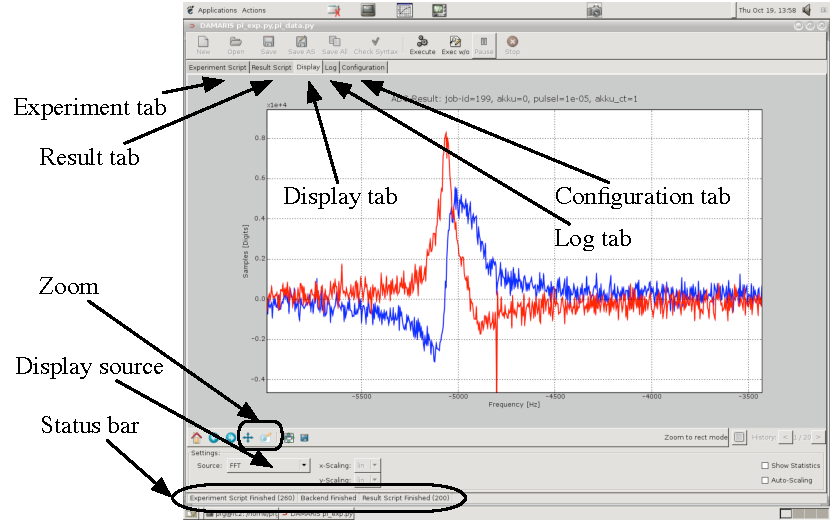
\includegraphics[]{damaris_description}
\caption{The \textsf{DAMARIS} front end}
\label{damarisoverview}
\end{figure}
The front end is composed of five tabs (Figure \ref{damarisoverview}): Experiment, Result, Display, Log and Configuration. This introduction into \textsf{DAMARIS} will begin with a NMR ``Hello World'' program, i.e. recording a FID. More elaborated techniques like phase cycling and PFG will be discussed in chapter \ref{advanced}.
\subsection{Configuration}
\begin{figure}[htbp]
\centering
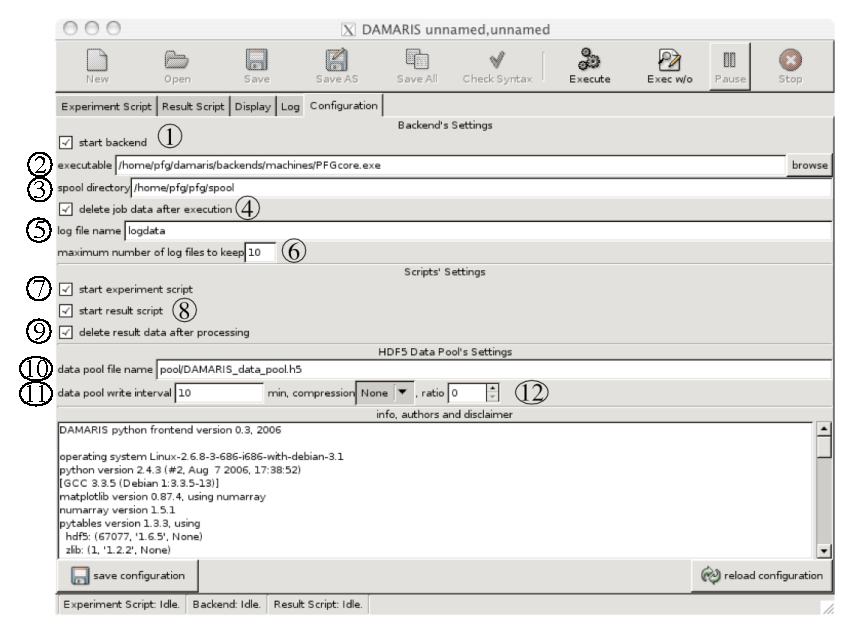
\includegraphics[]{config1}
\caption{Configuration tab}
\label{config}
\end{figure}
The Configuration tab  (Figure \ref{config}) offers a convenient way to setup \textsf{DAMARIS}. 
Following is a short description of the options:
\begin{enumerate}

\item Toggle the start  of the back end
\item Path to the back end executable, here \textbf{PFGcore.exe}
\item Path to the spool directory, where the job files will be written or picked up
\item Delete the job files after execution
\item Filename of the logfile 
\item Number of logfiles to keep
\item Toggle the start of the experiment script
\item Toggle the start of the result script
\item Toggle the deletion of results after they have been processed by the result script (see \ref{tuning})
\item Filename of the data pool file
\item Write interval after which the data pool is rewritten
\item Compression settings (see page \pageref{comp})
\item Authors, License and version numbers of used components
\end{enumerate}

\subsection{Experiment Script}
\lstinputlisting[caption=Experiment script for recording a FID]{codesnippets/FID_exp.py}
On the first line, the basic Experiment module is imported which loads the methods and commands to control an experiment. Next, a function \textbf{fid\_experiment} is defined which will contain everything necessary to run a single scan.
The first line inside the function creates an object \textbf{e} in which the states will be written by subsequent application of methods to this experiment object. This sequence of states is then passed to the caller.
When the ``Execute'' (
\includegraphics[keepaspectratio, height=12pt]{execute_button}) button is pressed, the experiment script is scanned for a function called \textbf{experiment}.
Thus, to run \textbf{fid\_experiment}, the \textbf{experiment} function has to contain a call to the \textbf{fid\_experiment}. 

Behind the scenes is the experiment script that writes the state sequence from \textbf{fid\_experiment}, an \textsf{XML}\footnote{http://www.w3c.org/XML} file, into the spool directory and the back end is then executed. The back end is simply reads these files, translates  the contents to pulse programmer code and stores the generated code into the memory of the pulse card. Finally, the pulse program is executed. Then the results are written by the back end into the spool directory, where they are provided to the result script. In the result script, the function \textbf{result} is then executed.% located in the Result tab.

\subsection{Result Script}
The function \textbf{result} in the result tab defines what should be done with the results. Here is a short example how to display the recorded signal:
\lstinputlisting[caption=Result script which is displaying the result]{codesnippets/FID_data.py}
After pressing the ``Execute'' (
\includegraphics[keepaspectratio, height=12pt]{execute_button}) button to start the experiment, the Display tab is opened. With the drop down menu right to ``Source'' under the graph window one can choose which data should be displayed. This list is built dynamically by the data dictionary in the result script, where the key denotes the name to be shown and the value contains the data. In this example we overwrite the data in the key \textbf(Timesignal) on every scan with the new result.
There are now two possibilities to export the figure:
\begin{enumerate}
\item Saving the plot as a figure (EPS, PNG, JPEG and more) by pressing the button 
\includegraphics[keepaspectratio, height=12pt]{save_as_picture3} in the toolbar below the plot area
\item Saving the data of the plot as CSV file (comma separated values) by pressing the button 
\includegraphics[keepaspectratio, height=12pt]{save_as_csv} on the right side of the toolbar under the plot
\end{enumerate}
 
\section{Accumulation}\label{advanced}
Sometimes the detected signals intensity is low compared to the noise, and can therefore not be seen. A measure for the quality of the recorded signal is the signal-to-noise ratio (SNR) which is defined as the ratio of signal versus the standard deviation of the noise, i.e. noise strength. 
The SNR is improved by measuring the signal many times and averaging the recorded signals, also called accumulation.
In \textsf{DAMARIS} this can be achieved by creating a loop in the experiment script and accumulating the results in the result script.
\lstinputlisting[caption=Experiment script showing how to create a loop]{codesnippets/Accumulate_exp.py}
\lstinputlisting[caption=Result script accumulating the data]{codesnippets/Accumulate_data.py}

\section{Phase Cycling}
Artefacts due to channel imbalance in the receiver, inhomogeneity in the RF field and unwanted signals, for example primary echos, can be suppressed or cancelled out by cycling the phases \citep{Berger:2004vn} of the receiver and the RF pulses and then accumulating the signal.
\lstinputlisting[caption=Experiment script for phase cycling]{codesnippets/Phase_exp.py}
New in this script is the \textbf{set\_description} method and a parameter \emph{run} that is passed to the experiment. The  \textbf{set\_description} method is used to set descriptions and values important to the experimenter or to pass values to the result script. These descriptions are written into the \textsf{XML} job file and stored by the back end into the result file. In this way it is possible to pass values to the result script so the latter can act upon these. In this case the result is either added or subtracted to the accumulation variable.
\section{Changing Parameters}
\begin{wrapfigure}[]{l}{3.8cm}
\mbox{
\includegraphics[]{inversion_recovery}}
\end{wrapfigure}
Now, this script is modified to measure the longitudinal relaxation time $\textrm{T}_{1}$ by a so called inversion recovery experiment. Therefore the $\frac{\pi}{2}$-pulse is preceded by $\pi$-pulse both separated by the variable time $\tau$. The FID after the second pulse is recorded. In order to get a good signal, accumulation and phase cycling are implemented.
In the result script, the magnetization will be obtained and, together with the corresponding variable $\tau$, stored in an \textsf{ASCII} file for determination of $\textrm{T}_{1}$.
\lstinputlisting[caption=Experiment script illustrating the use of variables]{codesnippets/t1_exp.py}
\lstinputlisting[caption=Result script writing the amplitude and corresponding delay time $\tau$ between the pulses to a file]{codesnippets/t1_data.py}

\section{Data Handling}
To store the result for further data analysis one has several built-in possibilities in \textsf{DAMARIS}. One can store the results as \textsf{ASCII} file or as \textsf{HDF5}\footnote{http://www.hdfgroup.org/HDF5} file. Writing  an \textsf{ASCII} file is usable for smaller data-sets and a small number of experiments. 
\lstinputlisting[caption=Part of a result script for saving data into an \textsf{ASCII} file]{codesnippets/CSVwrite.py}
\begin{figure}
\centering
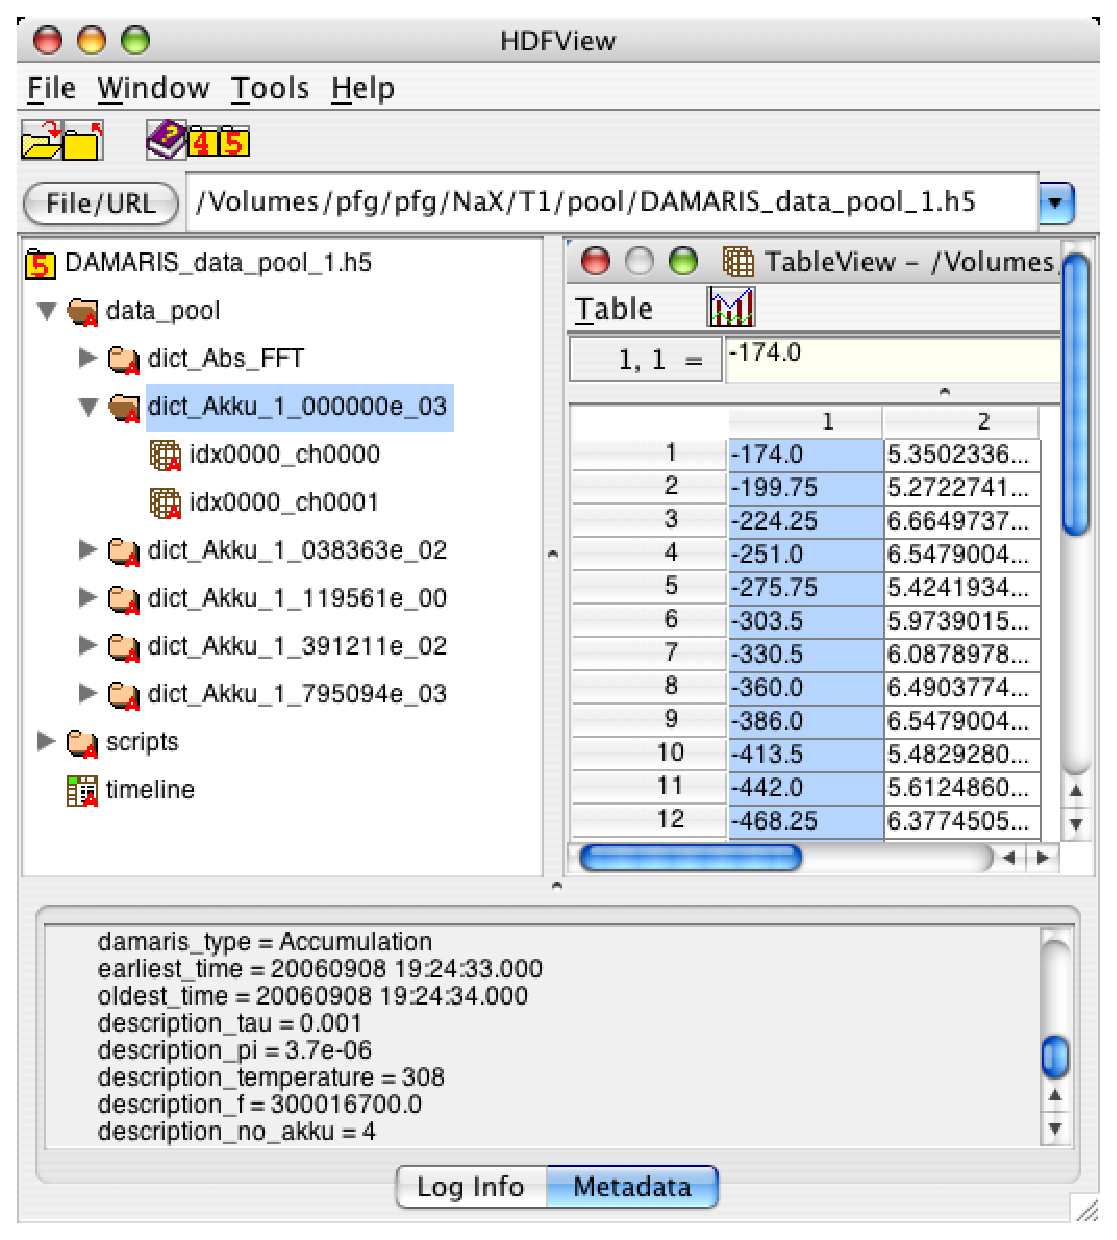
\includegraphics[scale=0.65]{result_file_t1} % war 0.5
\caption{A sample data pool file, opened with \textsf{HDFView}. On the bottom of the picture the metadata stored with the table can be seen}
\end{figure}
For bigger experiments it is advantageous to store data in a \textsf{HDF5} file. This is the \textsf{H}ierarchical \textsf{D}ata \textsf{F}ormat developed by the \textsf{NCSA} (\textsf{N}ational \textsf{C}enter for \textsf{S}upercomputer \textsf{A}pplications) for storing complex tables and big amounts of data in an effective way. It supports grouping of data, annotation and compression. A very convenient way to access \textsf{HDF} files in Python is the \textsf{pyTables} module, which is also used by \textsf{DAMARIS} internally. Another platform independent way to examine the results is the \textsf{HDFView} Java program provided by \textsf{NCSA}.

After an experiment in \textsf{DAMARIS} has been finished, the results in the data dictionary as well as the experiment and result scripts themselves are written automatically to a \textsf{HDF} file, the data pool file.\label{comp} In the configuration tab (Figure \ref{config}, 10-12), filename, compression ratio, compression library and write interval can be set up.
The write interval is the time after which the data pool file should be periodically rewritten and is useful in case of hardware failure. 
The results from the ADC are stored as 64-bit floating point values in tables which are compressed/decompressed  transparently/on-the-fly. 
In \textsf{DAMARIS}, three compression libraries are available: zlib, lzo and bz2. For a comparison of these, the \textsf{pyTables} homepage\footnote{http://pytables.sourceforge.net} offers a great wealth of information.
\textsf{HDFView} does not support viewing of bzip2 or lzo compressed data. In case the data has been compressed with lzo, the \emph{ptrepack} utility from \textsf{pyTables} can be used to recompress the data with zlib.

The speed-up in post-processing and analysis is already 24 fold in small data-sets with 32768 points per channel and 25 files on a Athlon XP 2600+ CPU with 512 MB RAM running Debian Sarge Linux. Thus, writing \textsf{HDF5} with compression enabled is highly recommended.

Note that in Listing \ref{advancedhdf} we create a \textsf{HDF5} file from scratch! Experiment and result script are not saved in the resulting file. The advantage is that one can create arbitrary complex structured files at the cost of having a more complicated result script.
\lstinputlisting[caption=Result script for saving data in a \textsf{HDF5} file, label=advancedhdf]{codesnippets/HDFwrite.py}
A very convenient and easier method to save data in HDF is the MeasurementResult class.
\begin{lstlisting}
...
def fid():
	# create a measurement object
	measurement=MeasurementResult("Magnetization(tau)")
	for timesignal in results:
		# extract "tau" from the description dictionary
		tau = timesignal.get_description('tau')
		...
		# get the magnetization from the timesignal
		magnetization = sqrt(timesignal.y[0][80:100].mean()**2 
						+ timesignal.y[1][80:100].mean()**2)
		measurement[tau] += magnetization
		# provide the magnetization curve
		data["Magnetization(tau)"] = measurement
		...
\end{lstlisting}
Essentially, a dictionary ``measurement'' is created with \emph{tau} as the key. For each new key the current magnetization is added. This dictionary is then added to the data pool. The advantage over Listing \ref{advancedhdf} is that the magnetization vs. $\tau$ curve can be directly displayed in order to gain an overview of the running experiment, because the ``measurement'' dictionary is added to the data pool. In this example, the value also stores statistics from the accumulation. The data dictionary is stored automatically as described before, including the result and experiment scripts, information about the used back end and a timeline of the experiment.

\section{Fourier Transform Module}
A module was written for an easy calculation of spectra from time domain data. The Fourier transformation module ``DamarisFFT'' is based on the \textbf{fft} module of \textbf{numpy}, an array module for Python. There are no interactive capabilities such as phase correction incorporated yet. The FFT method can be applied directly to the object (see Listing \ref{fftex}). The order in which these methods are applied \emph{does} matter. Here are the available methods and a short explanation of their effects is shown (values in italic are default values).
The change is \emph{in-place}, which means if the timesignal is needed later on, a copy of it should be made.

\begin{description}

\item[clip(start=\textit{None},stop=\textit{None})]
Only the data between start and stop is returned.
The start and stop parameters can be either in  time or frequency domain.

\item[baseline(lastpart=\textit{0.1})]
This method should be applied first as it corrects the baseline of the signal, taking the last \textbf{lastpart} part of the signal for determining the correction.

\item[autophase()]
This will try to automatically phase the spectrum to maximize the real signal. Works only reliably at sufficient high SNR (>20)

\item[fft(samples=\textit{None})]
This method returns the real and the imaginary part of an FFT of the timesignal. Zero-filling of the timesignal can be done via the \textbf{points} keyword. If \textbf{points} is bigger than the number of data points, the rest will be filled with zeros (zero-filling/zero-paddin


\item[abs\_fft(points=\textit{None})]
This method returns an absolute FFT of the timesignal. Zero-filling of the timesignal can be done via the \textbf{points} keyword. If \textbf{points} is larger than the number of data points, the rest will be filled with zeros (zero-padding). The \textbf{zoom} keyword accepts either a tuple with centre frequency and width in Hz. Auto zooming the highest peak can be achieved by setting the centre frequency to \textit{auto}.
g).
\end{description}
%
%\begin{itemize}
%\item realfft(points=None, zoom=None, write = 'off'):
%\end{itemize}
In order to suppress side-lobes, enhance resolution or improve SNR it is common practice in data processing to apply windowing functions to the data.
Several windowing functions are available in the ``DaFFT'' module. The first two functions, i. e. the exponential and gaussian window function are SNR enhancing windows, while the double exponential window function is resolution enhancing.
The TARF window is both, SNR and resolution enhancing\citep{Traficante:1987fk}.
 All four are commonly used in NMR spectroscopy. The line broadening factor LB is the rate (in Hz) in which the window function decays. The higher the value, the faster the function decays, hence the resulting spectrum will be more ``smooth'' but the peaks will become wider.

\begin{description}
\item[exp\_window(line\_broadening=\textit{10})]
This sets an exponential window over the data, the beginning of the signal is weighted more, where as the tail of the singal gets supressed. Best results are obtained with line broadening factor set to the peak width:
\begin{equation*}
f(x)=exp(-tp\cdot LB)
\end{equation*}

\item[gauss\_window(line\_broadening=\textit{10})]
This sets a gaussian window over the data:
\begin{equation*}
f(x)=exp(-(tp \cdot LB)^2)
\end{equation*}

\item[dexp\_window(line\_broadening=\textit{-10}, gaussian\_multiplicator=\textit{0.3}, show=\textit{0})]
This sets a double-exponential window over the data, which enhances the tail of the FID  thus prolonging it and increases the resolution. Note that the line broadening should have a negative value here. The reason is that weighting is supposed to increase from the beginning (exponential part) and then later to decrease again (gaussian part). Another point to mention is that this window is in fact transforming a lorentzian peak in a gaussian peak which has the property of a narrower base:
\begin{equation*}
f(x)=exp(-tp\cdot LB - GM\cdot  tp^2)
\end{equation*}

\item[traf\_window(line\_broadening=\textit{10})]
This sets a \textsf{TRAF} window \citep{Traficante:1987fk} over the data:
\begin{equation*}
f(x)=\frac{exp(-tp\cdot LB))^2} {\left[exp(-tp\cdot LB))^3 
                + (exp(-aq\_time\cdot LB)\right]^3 }
\end{equation*}

\end{description}
Following standard windowing functions \citep{Butz:1998fr} are available additionally. Note that the whole data will be windowed, not only a subset. Furthermore, these windows are not suitable for FID's or similar signals, because they are symmetric around the middle of the data set and zero at the beginning and the end. 
\begin{itemize}
\item hanning\_window()
\item hamming\_window()
\item blackman\_window()
\item bartlett\_window()
\item kaiser\_window(beta=4, show=0, use\_scipy=None)
\end{itemize}

To use this methods one has to apply consecutively the methods to an \emph{timesignal} or \emph{accumulation} object:
\begin{lstlisting}[label=fftex]
data["FFT"]=timesignal.baseline(0.4).exp_window(line_broadening=100).abs_fft().clip=(-1e3,1e3)
\end{lstlisting}

This applies baseline correction using the last 40\% of the timesignal for determination of the signal. Then, an exponential window is applied. From this timesignal an FFT is calculated which is furhter clipped to view to the data between \unit[-1]{kHz} with \unit[1]{kHz} width.

\section{Good Practices}
\begin{itemize}
\item Save often. It can become slow to open a \textsf{HDF} file in append mode and close it again for \emph{each} result, but in case of an error, the file is not completely lost.
\item Keep the experiment function simple. Everything necessary for a scan should be contained in a function, the parameters should stay in the \textbf{experiment} function. This makes it possible to loop over several parameters easier and, in case of complex experiments, all variables are changed in one place: the call to the function.
\item Display if necessary. If the repetition time of subsequent scans is short (several ms) it can slow down the result script notably. The result script will take care of this by not displaying every single shot, but displaying nothing would further speed up the processing of the results.
\item Save disk space. If the options ``delete results'' and ``delete jobs'' are switched off, the spool directory can get clobbered by several thousand files and  in the worst case, one can run out of \emph{inodes}. If it is not possible to delete the files in the directory anymore (rm gives an error ``too much arguments'') the following command  can help deleting the files anyway: 
\begin{quote}
\lstinline!find . -name job\* -exec rm {} \;!
\end{quote} which will delete all files starting with \textit{job} in the current directory.
\item It is a good idea to put a \emph{synchronize()} statement in the experiment script, for example after the 100th accumulation. This will write job files only until the synchronize is requested. Then, the front end will wait writing new job files, until the result script has processed all current results. In big experiments, several ten thousands job of files would be written without this, which can lead to problems with the file system and performance.
\begin{lstlisting}
if accu%100 == 0:
	synchronize()
\end{lstlisting}
\item Keep an eye on the logs. In case of errors it is highly recommended to check the log file in the log path (as defined in the configuration tab) \emph{as well} as the ``Log'' tab for error messages.
\end{itemize}


\section{Tuning and Development}
\label{tuning}
When new result scripts are developed, it is an advantage if the actual experiment has not to be repeated for every minor change or tweak in the result script. This can become a very tedious task when the sample has a long $\textrm{T}_{1}$ relaxation, like water $\textrm{T}_{1} \approx 3\textrm{s}$\citep{PhysRev.111.1201}. 
In order to use this technique, the experiment has to be run once with the option ``delete results after processing'' turned off. This leads to the result files in the spool directory not being deleted. Starting the experiment again with the option ``run back end'' switched off, the front end will read the results again like if it would be a new experiment, hence one can test new result scripts quite conveniently.
Developing experiment scripts can be done in a similar manner: the dummy back end  (to be set in the configuration tab) can be used to test new experiment scripts without the need to have a spectrometer at hand.
\section{Data Processing Outside \textsf{DAMARIS}}
For post-processing of the data, several options are available, depending on the format of the data. Most programs can handle \textsf{ASCII} files (\textsf{gnuplot}, \textsf{Origin}, fitsh, etc.), so this is the more flexible format. \textsf{HDF} can be read by \textsf{pyTables}, \textsf{Matlab}, \textsf{Octave}, \textsf{R}, \textsf{Mathematica} and more\footnote{http://hdf.ncsa.uiuc.edu/tools5desc.html}.



%%%%%%%%%%%%%%    Command    List     %%%%%%%%%%%%%%%%%%%%%
\section{List of Commands}
\subsubsection{Experiment Script Commands}
Following is a list of available commands in an experiment script.

\begin{description}

\item[ttl\_pulse(length, channel=\textit{None}, value=\textit{None})]
Gives out \emph{either} a \textsf{TTL} pulse with duration \textbf{length} on \textbf{channel} (counting from zero), \emph{or} multiple channels given by the binary representation of \textbf{value} (see Figure \ref{binary}).
\begin{figure}
\centering
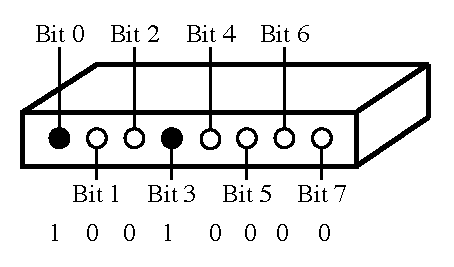
\includegraphics[]{pins_ttl_bit}
\caption{Line driver with a decimal value 17 set (or 0x11 hexadecimal). In binary, channel 0 and channel 3 are on}
\label{binary}
\end{figure}

%\newline

\emph{\textbf{Example}}:
\begin{lstlisting}
e.ttl_pulse(lenght=5e-6, channel=1)
e.ttl_pulse(lenght=3e-6, value=3)
\end{lstlisting}
This example is used to create a RF pulse with a pulse length of \unit[3]{$\mu$s}. The first statement sets the gate pulse (channel 0) of the RF amplifier for \unit[5]{$\mu$s}, while the second  statement combines the gate and RF pulse on channels 0 and 1 ($2^0 + 2^1 = 3$). Hexadecimal representation (number starts with \emph{0x}) is convenient as the numbers are shorter: To set all channels, \textbf{value} would be in decimal 16777215 and in hexadecimal 0xffffff. One letter in hexadecimal represents four bits.

\item[ttls(length=None, value=None)]
Same as \textbf{ttl\_pulse(length, value)}

\item[wait(time)]
Wait specified \textbf{time} in seconds. Minimum time is \unit[90]{ns}, maximum time is essentially  unlimited (years). The limit imposed from the pulse programmer is circumvented by the driver.
\newline
\emph{\textbf{Example}}:
\begin{lstlisting}
e.wait(length=2e-3)
\end{lstlisting}

\item[record(samples, frequency, timelength=\textit{None}, sensitivity=\textit{None})]
Records data with given number of \textbf{samples}, sampling-frequency \textbf{frequency} and \textbf{sensitivity} in Volts.
If \textbf{timelength} is given, this state will stay the given time. The maximum sampling-frequency is  \unit[20]{MHz} and the onboard memory can hold 8M samples shared by both channels. Sensitivity can be one of 0.2, 0.5, 1, 2, 5 and  \unit[10]{V}.
Not that multiple  record statements can be in a single scan (gated sampling) or in a loop.
\newline
\emph{\textbf{Example}}:
\begin{lstlisting}
e.record(samples=1024, frequency=2e6, sensitivity=2)
\end{lstlisting}
Records a signal with 1024 data points and \unit[2]{MHz} sampling-frequency. The sensitivity will be $\pm$ \unit[2]{V}. With a 14bit ADC  card this gives a resolution of  \unit[0.2]{mV}. 

%\item[state\_start(time)/ state\_end()]
%Starts a state for a given \textbf{time} and should be closed by a state\_end() command.
%\newline
%\emph{\textbf{Example}}:
%\begin{lstlisting}
%e.state_start(time=10e-3)
%e.rf_pulse(channel=1)
%e.state_end()
%\end{lstlisting}
%This will give a pulse for 10 ms on channel 0.

\item[loop\_start(iterations)/loop\_end()]
This creates a loop of given number of \textbf{iterations} and has to be closed by loop\_end().
Commands inside the loop can not change, i.e. the parameters are the same for each loop run. This loop is created on the pulse programmer, thus saving commands.
\newline
\emph{\textbf{Example}}:
\begin{lstlisting}
e.loop_start(iterations=10)
e.rf_pulse(channel=3, length=2e-6) 
e.wait(time=2e-6)
e.loop_end()
\end{lstlisting}
This loop will create 10 pulses with \unit[2]{$\mu$s} length and \unit[2]{$\mu$s} apart.

\item[set\_frequency(frequency, phase, ttls=\textit{0})]
Sets the \textbf{frequency} and \textbf{phase} of the frequency source and optionally further channels. The time needed to set the frequency is \unit[2]{$\mu$s}.
\newline
\emph{\textbf{Example}}:
\begin{lstlisting}
e.set_frequency(frequency=300.01e6, phase=0)
\end{lstlisting}
The frequency generator wil deliver  \unit[300.01]{MHz}.
\begin{lstlisting}
e.set_frequency(frequency=300.01e6, phase=0, ttls=3)
\end{lstlisting}
Same as above, but also sets channel 0 and 1.

\item[set\_phase(phase, ttls=\textit{0})]
This command can be used to change the phase of the frequency. The \textit{phase} is given in degree. The \textsf{ttls} keyword has the same functionality like in the set\_frequency command. Setting the phase is done  in \unit[0.5]{$\mu$s}
\newline
\emph{\textbf{Example}}:
\begin{lstlisting}
e.set_phase(phase=90)
e.record(samples=1024, frequency=2e6, sensitivity=2)
\end{lstlisting}
This would set the receiver phase to 90 degree.
\item[set\_pts\_local()]
If the frequency source is set to remote control mode, this can be used to set to local mode, thus the frequency of the PTS synthesizer can be changed manually.
%\end{description}
%\begin{description}
\item[set\_pfg(length, dac\_value, shape=('rec',0), trigger=4, is\_seq=\textit{0})]
With this command, pulsed field gradients are generated. In order to create arbitrary ramps or shapes, \textbf{is\_seq} can be set to 1, leading the DAC to to keep the current state until a new strength is applied.
The trigger keyword allows to set a trigger line with the start of the gradient pulse.
Certain gradient shapes are predefined:
\begin{itemize}
\item rectangular ('rec')
\item $\mathsf{sin}$ ('sin')
\item $\mathsf{sin}^2$ ('sin2')
\end{itemize}
You can select them by giving the shape keyword a tuple with shape and resolution in s
\emph{\textbf{Example}}:
\begin{lstlisting}
e.set_pfg(length=1e-3, dac_value=15040, is_seq=0)
\end{lstlisting}
This would create a \unit[1]{ms} long PFG pulse with \unit[1]{$\textrm{Tm}^{-1}$}
\begin{lstlisting}
for val in lin_range(start=0, stop=pi, step=pi/50):
	gradient = int( sin(val)**2 * 15040 )
	e.set_pfg(length=1e-3/50, dac_value=gradient, is_seq=1)
\end{lstlisting}
This would create a \unit[1]{ms} long PFG pulse shaped like half period of a $\sin^2$ with an amplitude of \unit[1]{$\textrm{Tm}^{-1}$}.

\begin{lstlisting}
e.set_pfg(length=1e-3, dac_value=15040, shape=('sin2', 1e-5))
\end{lstlisting}
This would create a  $\mathsf{sin}^2$ shaped gradient with 1ms length and 100 interpolation points.


%\item[set\_pfg\_wt(length, dac\_value, is\_seq=\textit{0}, trigger=\textit{4})]
%Same as above, but with an additional ttl pulse for use as a trigger for an oscilloscope. This is a convenient method for monitoring gradients.
%\newline
%\emph{\textbf{Example}}:
%\begin{lstlisting}
%e.set_pfg_wt(length=1e-3, dac_value=15040, is_seq=0, trigger=4)
%\end{lstlisting}
%This would allow it to monitor the current monitor of the current supply with an oscilloscope using an external trigger.

\item[set\_description(key, value)]
Setting a description is accomplished by this command. It creates an entry  \textbf{key} with value \textbf{value} in the description dictionary\footnote{see get\_description in result script commands on how to access it}. In case of the data being stored in a \textsf{HDF5} file this dictionary is stored as well. 
\newline
\emph{\textbf{Example}}:
\begin{lstlisting}
e.set_description(key="tau", value=2e-3)
\end{lstlisting}
%\newline
\end{description}
Following are convenient functions for use in loops.


\begin{description}

\item[lin\_range(start, stop, step)] This is used for loops. It increases \textbf{start} with \textbf{step} until \textbf{stop} is reached.
\newline
\emph{\textbf{Example}}:
\begin{lstlisting}
def experiment():
	for tp in lin_range(start=5e-7, stop=10e-6, step=5e-7):
		yield pi_pulse(pulselength=tp)
\end{lstlisting}
Starting from \unit[0.5]{$\mu$s}, increase pulse length with \unit[0.5]{$\mu$s} until \unit[10]{$\mu$s}.



\item[log\_range(start, stop, stepno)] Divide the range \textbf{start} to \textbf{stop} logarithmically in \textbf{stepno} steps.
\newline
\emph{\textbf{Example}}:
\begin{lstlisting}
def experiment():
	for t in log_range(start=5e-3, stop=10, stepno=10):
		yield inversion_recovery(tau=t)
\end{lstlisting}
Variate the distance $\tau$ of the two pulses in the inversion recovery experiment logarithmically from \unit[5]{ms} to \unit[10]{s}. The values would be:
['0.0050', '0.0116', '0.0271', '0.0630', '0.1466', '0.3411',
       '0.7937', '1.8469', '4.2975', '10.0000']
       
       
\item[staggered\_range(some\_range, size=\textit{1})] Creates a staggered range from another range, leaving out \textbf{size} values in a row and appending the left  out  later.
\newline
\emph{\textbf{Example}}:
\begin{lstlisting}
def experiment():
	myrange=log_range(start=5e-3, stop=10, stepno=10)
	for tp in staggered_range(myrange, size=2):
		yield inversion_recovery(tau=t)
\end{lstlisting}
This is the same as before, but the values are now staggered: 12345678 will become 12563478. Another possibility for achieving something similar is the \emph{shuffle} function (see Listing \ref{naxexp}).

\item[interleaved\_range(some\_range, size=\textit{1})] Creates an interleaved range from another range, appending every n-th point.
\newline
\emph{\textbf{Example}}:
\begin{lstlisting}
def experiment():
	myrange=log_range(start=5e-3, stop=10, stepno=10)
	for tp in interleaved_range(myrange, size=3):
		yield inversion_recovery(tau=t)
\end{lstlisting}

The values are now interleaved: 12345678 will become 14725836. Another possibility for achieving something similar is the \emph{shuffle} function (see Listing \ref{naxexp}).


\item[combine\_ranges(*ranges)] With this function it is possible to combine several ranges 
\newline
\emph{\textbf{Example}}:
\begin{lstlisting}
def experiment():
	mylinrange=lin_range(start=1e-3, stop=4.9e-3, step=1e-4)
	mylogrange=log_range(start=5e-3, stop=10, stepno=10)
	for tp in combine_ranges(mylinrange, mylogrange):
		yield inversion_recovery(tau=t)
\end{lstlisting}

%\item[get\_job\_id()]
%Returns the job id of the current running job
%\item[write\_xml\_job()]
%Returns a xml job which can be saved in a file
%\item[write\_quit\_job()]
%Returns a quit job.

\end{description}

\subsubsection{Result Script Commands}
Following is a list of available commands in a result script. These are methods to be applied to a ADC\_Result and  Accumulation  object. An accumulation object needs to be created before any methods can be applied.
\newline
\emph{\textbf{Example}}:
\begin{lstlisting}
akku = Accumulation(error=True)
akku += timesignal
\end{lstlisting}

\begin{description}
%ADC\_Result
\item[get\_result\_by\_index(index)] 
If several \textbf{record} statements occur in an experiment, the results are saved in an array and can be accessed by this method. \textit{Index} starts with 0.
\newline
\emph{\textbf{Example}}:
\begin{lstlisting}
timesignal.get_result_by_index(1)
\end{lstlisting}
This would return the result of the second record statement.
\item[get\_sampling\_rate()]
Returns ADC card sampling rate
\item[uses\_statistics()]
Returns \textit{False} if the result is a single ADC result and \textit{True} if the result is an accumulation with statistics enabled.
\item[write\_to\_csv(destination=\textit{sys.stdout})]
Writes the result into an ASCII file, destination has to be an open file. The file has to be closed after write\_as\_csv has been  issued otherwise the data is not written to the harddrive.
\newline
\emph{\textbf{Example}}:
\begin{lstlisting}
f = open('testfile.dat' , 'w')
timesignal.write_to_csv(destination=f)
f.close()
\end{lstlisting}
\item[write\_to\_hdf(hdffile, where, name, title, compress=\textit{None})]
Writes the data to a HDF5 file \textbf{hdffile}.
%resultable
\item[get\_job\_id]
%\item[get\_description\_dictionary()]
%\item[set\_description\_dictionary(dictionary)]
\item[get\_description(key)]
Returns \textbf{value} of description \textbf{key} as string. Note that in the case of application to an accumulation object, only the common descriptions are stored, leading to a proper set of relevant parameters.
%\item[set\_description(key, value)]
%Drawable
\item[get\_xdata()]
Returns a copy of timedata.
\item[set\_xdata(pos, value)]
\item[get\_ydata(channel)]
Returns a copy of the data from channel \textbf{channel}
\item[set\_ydata(channel, pos, value)]
\item[get\_number\_of\_channels()]
Retuns the number of ADC channels, usually 2
\item[get\_xlabel()/get\_ylabel()]
Returns the x/y-axis description in display register
\item[set\_xlabel(label)/set\_ylabel(label)]
Sets the label of the x/y-axis
\item[get\_text(index)]
Returns labels to be plotted (List)
\item[set\_text(index, text)]
Sets labels to be plotted
\item[get\_title()]
Returns the title of the plot
\item[set\_title(title)]
Sets the title of the plot
\item[get\_legend()]
Returns the legend of the plot (dictionary)
\item[set\_legend(channel, value)]
Sets the legend of the plot
\item[get\_xmin()]
Returns minimum of x
%\item[set\_xmin(xmin)]
%Sets minimum of x
\item[get\_xmax()]
Returns maximum of x
%\item[set\_xmax(xmax)]
%Sets maximum of x
\item[get\_ymin()]
Returns minimun of y
%\item[set\_ymin(ymin)]
%Sets minimum of y
\item[get\_ymax()]
Returns maximum of y
%\item[set\_ymax(ymax)]
%Sets maximum of y
\end{description}


\newpage
\chapter{\textsf{DAMARIS} for Developers}
\label{damarisdev}
This chapter is dealing with the internals of \textsf{DAMARIS}. After an introduction of the back end, it is described how the Tecmag DAC20 driver is operating and how it has been implemented into \textsf{DAMARIS}. The complete source code of \textsf{DAMARIS} is available in a subversion\footnote{http://svnbook.red-bean.com} source repository for convenient access at \newline http://www.fkp.physik.tu-darmstadt.de/damaris.
\section{The Back End}
Starting the back end is causing it to search in the given spool directory for \textsf{XML} job files. These numbered files are containing a sequence composed of states, which themselves contain instructions for the experiment, or sub-sequences (which can contain further states or sub-sequences and can be looped).
%\begin{floatingfigure}{5.2cm}
%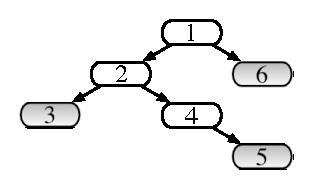
\includegraphics[]{traversing}
%\caption{Traversing of the state tree: shaded elements are states, white ones are sequences}
%\end{floatingfigure}
A state defines the output (24 bits) of the pulse programmer and can be either empty or contain sub-elements (state atoms), which for example could be an instruction to set a channel on the pulse programmer or set the DAC for a PFG current source.

\begin{wrapfigure}[]{l}{2.8cm}
\mbox{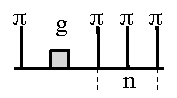
\includegraphics[]{devsequence}}
\end{wrapfigure}
The back end examines this \textsf{XML} job files and traverses the state sequence. Encountering a sub-sequence, this is traversed to its end, where the back end jumps out of the sub-sequence and continues where it entered the sub-sequence. This traversing is called \emph{depth-first}, and causes this nested \emph{state tree} to be processed sequentially in order (Figure \ref{traverseex}).
As an example the pulse sequence $\pi$-wait-pfg-wait-$\pi$-(wait-$\pi$-wait-$\pi$)n will be explained in depth. Once this pulse sequence is written in the \textsf{DAMARIS} front end, it results in a \textsf{XML} file (Listing \ref{jfwl}).
\lstinputlisting[language=xml, label=jfwl, caption="\textsf{XML} job containing a loop"]{codesnippets/jobfile_with_loop.xml}
\begin{figure}
\centering
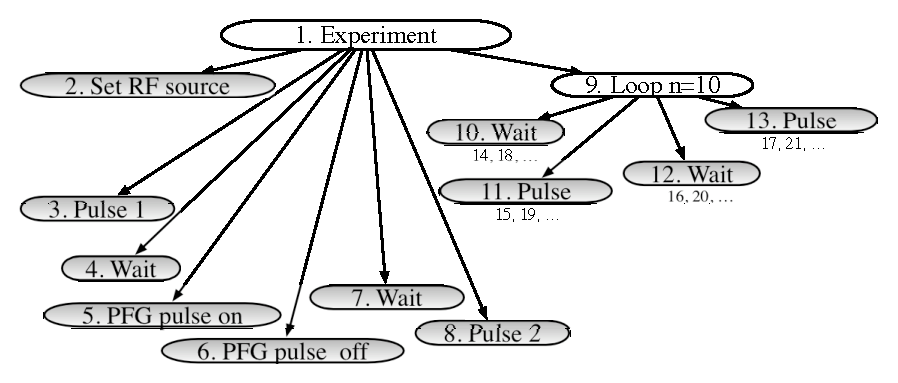
\includegraphics[]{traversing_example}
\caption{The \textsf{XML} file (Listing \ref{jfwl}) represented as a state tree. Elements are numbered in the order of the traversing. The loop is only traversed once, despite that the elements inside the loop will be executed repeatedly in the experiment. }
\label{traverseex}
\end{figure}
Each driver in the back end (PTS synthesizer, PFG, etc.) is traversing this tree, searching for elements it is responsible for. The driver then translates these elements in pure states for the pulse programmer (Figure \ref{traversemachine}), i.e. TTL  signals. Then, the next driver is traversing the tree, translating the elements it is responsible for. This is going on until all elements from the tree are translated into states, which are then written in machine code to the pulse programmer and executed.
\begin{figure}
\centering
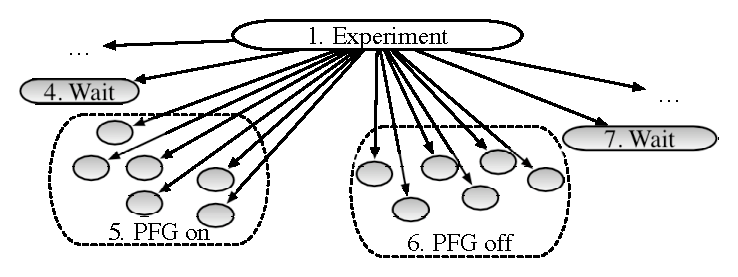
\includegraphics[]{traversing_machine}
\caption{Part of the state tree where the element of the state dealing with PFG was translated}
\label{traversemachine}
\end{figure}
Any result obtained by the back end is written to the corresponding \textsf{XML} result file (job filename + .result).
%\lstinputlisting[language=XML,caption=Example for a \textsf{XML} job file from a PFG spin echo experiment]{codesnippets/job.000054085}

\section{The DAC driver}
%\begin{floatingfigure}{6.5cm}
%\centering
%\mbox{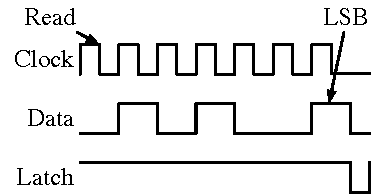
\includegraphics[]{dacword}}
%\caption{Transferring a DAC word}
%\end{floatingfigure} 
If in a state an \emph{analogout} element with suitable ID is encountered, the DAC driver  extracts the integer value for the gradient strength. The integer value is translated to binary representation (Listing \ref{daccode}, lines 133-141), and the single bits are transferred to the DAC (Listing \ref{daccode}, lines 160-190). Then, the time of the state is shortened by the time needed to transfer the complete data to the DAC. Every pulse necessary for transferring the data is created by the pulse programmer.
Transferring the data to the DAC is achieved by three lines, notably LE (latch enable), CLK (clock signal) and DATA (data line). Reading in a DAC word goes as follows: LE stays high, a data bit is read in with the falling edge of the clock signal, i.e. CLK high to CLK low. After the last (20th) bit is recorded, LE is going low thus signaling the DAC that the word is complete.
\lstinputlisting[label=daccode ,language=c++, linerange={117-191}, caption=Main logic of the DAC driver]{codesnippets/DAC20_tabbed.cpp}
This procedure was first tested and further refined in Python. Embeding the driver properly in the \textsf{DAMARIS} back end  made it necessary to translate the test program to \textsf{C++} \citep{Stroustrup:2000fk} code. The following files of the back end needed to be modified or created:
\begin{itemize}
\item drivers/pfggen.h
\item drivers/Tecmag-DAC20/DAC20.cpp
\item drivers/Tecmag-DAC20/DAC20.h
\end{itemize}
These three files are the main part of the driver. They contain the main logic for the DAC serial line.
%\begin{itemize}
%\item core/job.cpp
%\item core/job.h
%\item core/states.h
%\item core/xml\_states.cpp
%%\item drivers/Tecmag-DAC20/xmltest.xml
%\end{itemize}
%Here are the files which are parsing the \textsf{XML} file and extracting the information like dac\_value and length out of it. Only minor modifications needed to be done here.
\begin{itemize}
\item machines/hardware.cpp
\item machines/hardware.h
\item machines/PFGcore.cpp
\end{itemize}
Finally, these last files contain the spectrometer setup information, i.e. which frequency synthesizer, ADC card, pulse programmer or temperature controller is used. The resulting PFGcore.exe is the back end which is executed by the front end and has to be specified in the configuration tab.
\lstinputlisting[language=c++, caption=PFGcore.cpp which defines the spectrometer hardware]{codesnippets/PFGcore.cpp}

In the front end the following file needed to be modified to be able to use the PFG conveniently:
\begin{itemize}
\item Experiment.py
\end{itemize}
This file contains the functions to create a pulse sequence. The command \textbf{set\_pfg}, which adds the proper \textsf{XML} element to the state tree, has been added.
\begin{lstlisting}
...

def set_pfg(self, I_out=None, dac_value=None, length=None, is_seq=0):
	"""This sets the value for the PFG, it also sets it back automatically.
	If you don't whish to do so (i.e. line shapes)  set is_seq=1"""
	if I_out != None:
		print "I_out is deprecated"
	if I_out == None and dac_value == None:
	    dac_value=0
	if I_out != None and dac_value == None:
	    dac_value=dac.conv(I_out)
	if I_out == None and dac_value != None:
	    dac_value=dac_value
	if I_out !=None and dac_value != None:
	    dac_value = 0
	    print "WARNING: You can't set both, I_out and dac_value! dac_value set to 0"
	if length == None:
	    # mimimum length
	    length=42*9e-8
	self.state_list.append('<state time="%s">
					  <analogout id="1" dac_value="%i"/>
					  </state>\n' %(repr(length), dac_value))
	if is_seq == 0:
	    # Set the DAC back to zero if this is not part of a sequence 
	    self.state_list.append('<state time="%s">
					      <analogout id="1" dac_value="0"/>
					      </state>\n' %(repr(42*9e-8)) )
 ...
\end{lstlisting}
The conversion factor is \unit[50]{$\textrm{AV}^{-1}$}. The DAC receives the data from the pulse card after the signals are brought into rectangular shape by the cable driver. The bipolar signal is digitally encoded in 2s-complement , i.e. one bit represents the sign of the integer, thus the range of integer values starts from $\mathrm{-2^{19}}$ to $\mathrm{2^{19}-1}$. 
The DAC outputs a voltage according to the DAC word until the DAC receives another value. This behavior is important to the experimenter because if one wants to set a value only for a certain time it is necessary to set the value back to zero. In the \textsf{DAMARIS} front end this is done automatically with \textbf{set\_pfg}(dac\_value, length) whereas in the back end it is done at the beginning of each experiment to protect the hardware and to set the DAC into an defined state. 
Arbitrary shaping of gradient pulses is also possible by using the command \textbf{set\_pfg}(\textit{dac\_value}, \textit{length}, \textit{isseq}=1) which prevents setting the DAC to zero after the given length. Through concatenating subsequently \textbf{set\_pfg}(dac\_value, length, isseq=1) commands one can create almost any possible shape and/or background gradients. 
Shaping the gradients was not the focus of this work but the general function was tested using an oscilloscope at the current monitor of the PFG current source with the DAC creating a sine wave using several resolutions (Figure \ref{shapegrad}).
\begin{figure}[h]
\centering
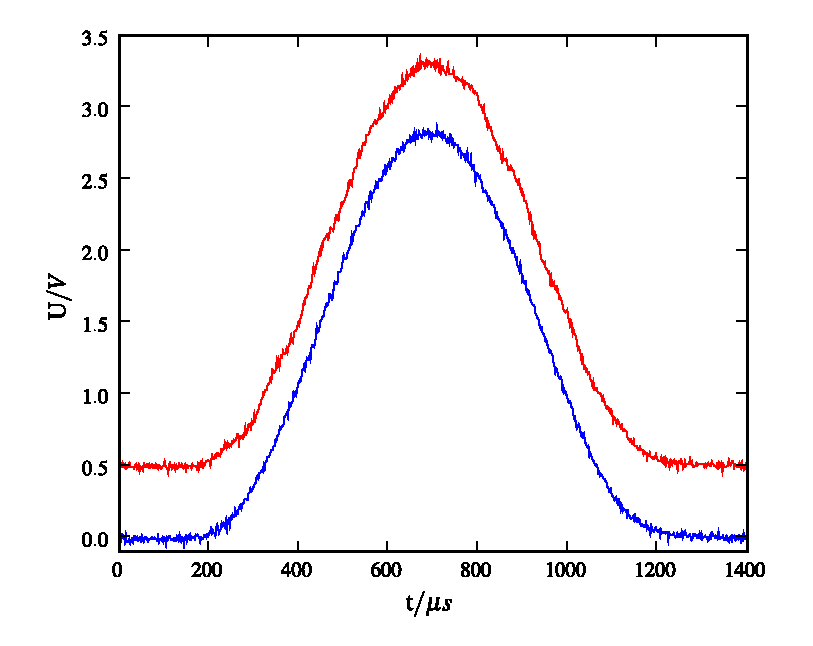
\includegraphics[]{pics/shapegrad1}
\caption{A $\sin^2$  PFG pulse with \unit[1]{ms} length. The upper one with \unit[100]{$\mu$s}, the lower one with \unit[3.78]{$\mu$s} resolution }
\label{shapegrad}
\end{figure}



%\begin{floatingfigure}{\textwidth}
\begin{figure}[ht]
\centering
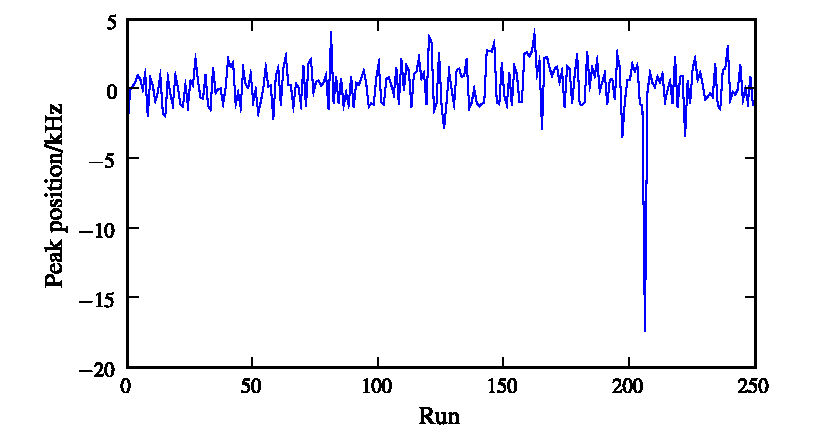
\includegraphics[]{pics/dac_fc}
\caption{The DAC is controlling the $B_{0}$ field and the peak position of the FFT signal has been recorded. For each signal the DAC is newly set to the same value. The time delay between each scan is \unit[50]{s} }
\label{gradstability}
\end{figure}
%\end{floatingfigure}
Theoretical resolution is given by approximately $\textrm{280A}/\textrm{2}^{\textrm{19}}$=\unit[0.000534]{A}. Tranfering in a 20bit word needs 21 cycles where each clock cycle is \unit[180]{ns} long. This leads to a time resolution of \unit[3.78]{$\mu$s}. Note that each DAC setting needs 42 instructions which can lead to problems regarding the memory of the PulseBlaster in the case of gradient pulse shaping. In Figure \ref{shapegrad},  the lower gradient, the maximum time resolution of \unit[3.78]{$\mu$s} was used, there are 264 steps, each of them with 42 states leading to more than 11.000 instructions for this pulsed field gradient alone. 

An improvement would be the use of loops for repeating patterns in the DAC word. The easiest approach would be  counting consecutively ones and zeros and write a loop if a one or a zero is repeated, i.e. so called \emph{run-length compression}. Even better would be searching for general patterns and use the best (in respect to memory, the smallest) instruction set. Another way to save instructions is to save the shape as a subprogram on the pulse programmers memory and recall it when it is needed. This possibility is not yet implement in the pulse programmer driver.

Stability of the DAC has been tested by measuring the shifts of resonance frequency in a Field Cycling spectrometer where the DAC controlled the magnetic field (Figure \ref{gradstability}). The DAC was very stable and the standard deviation of the frequency shift was about \unit[3]{kHz} and no drifts were visible except for one outlier which is good compared to the usual \unit[6]{kHz}\footnote{Value in the laboratoy book} with the standard field cycling DAC. Further stability measurements using an \textsf{Agilent 3440 A} high resolution multimeter have been also preformed. These measurements lead to the conclusion that the DAC is sufficiently stable and temperature drifts do not occur.

The offset of the PFG amplifier was adjusted via the offset potentiometer on the DAC board. There is also an offset adjustment possible at the PFG amplifier directly. For adjustment, the signal of water in a sample tube with a \unit[0.5]{mm} teflon stripe perpendicular to the magnetic field $B_{0}$ was recorded. First, the PFG power supply has been switched off and the sample was shimmed with the room temperature shims until the longest decay time $T^\ast_{2}$ of the FID has been  achieved. After this, the PFG was switched on and the offset has been adjusted to cause least distortion in the spectrum.

\chapter{Scripts for Various Experiments}
\lstinputlisting[caption=Experiment script for measuring diffusion in NaX with 13 interval pulse sequence, label=naxexp]{codesnippets/NaX_exp.py}
\newpage
\lstinputlisting[caption=Result script for measuring diffusion in NaX with 13 interval pulse sequence, label=naxdata]{codesnippets/NaX_data.py}
%
%\chapter{DaFFT Module}
%\lstinputlisting[caption=Source code of the DaFFT module for calculating spectra in \textsf{DAMARIS}]{codesnippets/DaFFT.py}
%

\bibliography{bibdesk_db}

\end{document}
 
